\documentclass[a4paper,12pt,twoside]{memoir}

% Castellano
\usepackage[spanish,es-tabla]{babel}
\selectlanguage{spanish}
\usepackage[utf8]{inputenc}
\usepackage[T1]{fontenc}
\usepackage{lmodern} % Scalable font
\usepackage{microtype}
\usepackage{placeins}

\RequirePackage{booktabs}
\RequirePackage[table]{xcolor}
\RequirePackage{xtab}
\RequirePackage{multirow}

% Links
\PassOptionsToPackage{hyphens}{url}\usepackage[colorlinks]{hyperref}
\hypersetup{
	allcolors = {red}
}

% Ecuaciones
\usepackage{amsmath}

% Rutas de fichero / paquete
\newcommand{\ruta}[1]{{\sffamily #1}}

% Párrafos
\nonzeroparskip

% Huérfanas y viudas
\widowpenalty100000
\clubpenalty100000

% Imágenes

% Comando para insertar una imagen en un lugar concreto.
% Los parámetros son:
% 1 --> Ruta absoluta/relativa de la figura
% 2 --> Texto a pie de figura
% 3 --> Tamaño en tanto por uno relativo al ancho de página
\usepackage{graphicx}
\newcommand{\imagen}[3]{
	\begin{figure}[!h]
		\centering
		\includegraphics[width=#3\textwidth]{#1}
		\caption{#2}\label{fig:#1}
	\end{figure}
	\FloatBarrier
}

% Comando para insertar una imagen sin posición.
% Los parámetros son:
% 1 --> Ruta absoluta/relativa de la figura
% 2 --> Texto a pie de figura
% 3 --> Tamaño en tanto por uno relativo al ancho de página
\newcommand{\imagenflotante}[3]{
	\begin{figure}
		\centering
		\includegraphics[width=#3\textwidth]{#1}
		\caption{#2}\label{fig:#1}
	\end{figure}
}

% El comando \figura nos permite insertar figuras comodamente, y utilizando
% siempre el mismo formato. Los parametros son:
% 1 --> Porcentaje del ancho de página que ocupará la figura (de 0 a 1)
% 2 --> Fichero de la imagen
% 3 --> Texto a pie de imagen
% 4 --> Etiqueta (label) para referencias
% 5 --> Opciones que queramos pasarle al \includegraphics
% 6 --> Opciones de posicionamiento a pasarle a \begin{figure}
\newcommand{\figuraConPosicion}[6]{%
  \setlength{\anchoFloat}{#1\textwidth}%
  \addtolength{\anchoFloat}{-4\fboxsep}%
  \setlength{\anchoFigura}{\anchoFloat}%
  \begin{figure}[#6]
    \begin{center}%
      \Ovalbox{%
        \begin{minipage}{\anchoFloat}%
          \begin{center}%
            \includegraphics[width=\anchoFigura,#5]{#2}%
            \caption{#3}%
            \label{#4}%
          \end{center}%
        \end{minipage}
      }%
    \end{center}%
  \end{figure}%
}

%
% Comando para incluir imágenes en formato apaisado (sin marco).
\newcommand{\figuraApaisadaSinMarco}[5]{%
  \begin{figure}%
    \begin{center}%
    \includegraphics[angle=90,height=#1\textheight,#5]{#2}%
    \caption{#3}%
    \label{#4}%
    \end{center}%
  \end{figure}%
}
% Para las tablas
\newcommand{\otoprule}{\midrule [\heavyrulewidth]}
%
% Nuevo comando para tablas pequeñas (menos de una página).
\newcommand{\tablaSmall}[5]{%
 \begin{table}
  \begin{center}
   \rowcolors {2}{gray!35}{}
   \begin{tabular}{#2}
    \toprule
    #4
    \otoprule
    #5
    \bottomrule
   \end{tabular}
   \caption{#1}
   \label{tabla:#3}
  \end{center}
 \end{table}
}

%
% Nuevo comando para tablas pequeñas (menos de una página).
\newcommand{\tablaSmallSinColores}[5]{%
 \begin{table}[H]
  \begin{center}
   \begin{tabular}{#2}
    \toprule
    #4
    \otoprule
    #5
    \bottomrule
   \end{tabular}
   \caption{#1}
   \label{tabla:#3}
  \end{center}
 \end{table}
}

\newcommand{\tablaApaisadaSmall}[5]{%
\begin{landscape}
  \begin{table}
   \begin{center}
    \rowcolors {2}{gray!35}{}
    \begin{tabular}{#2}
     \toprule
     #4
     \otoprule
     #5
     \bottomrule
    \end{tabular}
    \caption{#1}
    \label{tabla:#3}
   \end{center}
  \end{table}
\end{landscape}
}

%
% Nuevo comando para tablas grandes con cabecera y filas alternas coloreadas en gris.
\newcommand{\tabla}[6]{%
  \begin{center}
    \tablefirsthead{
      \toprule
      #5
      \otoprule
    }
    \tablehead{
      \multicolumn{#3}{l}{\small\sl continúa desde la página anterior}\\
      \toprule
      #5
      \otoprule
    }
    \tabletail{
      \hline
      \multicolumn{#3}{r}{\small\sl continúa en la página siguiente}\\
    }
    \tablelasttail{
      \hline
    }
    \bottomcaption{#1}
    \rowcolors {2}{gray!35}{}
    \begin{xtabular}{#2}
      #6
      \bottomrule
    \end{xtabular}
    \label{tabla:#4}
  \end{center}
}

%
% Nuevo comando para tablas grandes con cabecera.
\newcommand{\tablaSinColores}[6]{%
  \begin{center}
    \tablefirsthead{
      \toprule
      #5
      \otoprule
    }
    \tablehead{
      \multicolumn{#3}{l}{\small\sl continúa desde la página anterior}\\
      \toprule
      #5
      \otoprule
    }
    \tabletail{
      \hline
      \multicolumn{#3}{r}{\small\sl continúa en la página siguiente}\\
    }
    \tablelasttail{
      \hline
    }
    \bottomcaption{#1}
    \begin{xtabular}{#2}
      #6
      \bottomrule
    \end{xtabular}
    \label{tabla:#4}
  \end{center}
}

%
% Nuevo comando para tablas grandes sin cabecera.
\newcommand{\tablaSinCabecera}[5]{%
  \begin{center}
    \tablefirsthead{
      \toprule
    }
    \tablehead{
      \multicolumn{#3}{l}{\small\sl continúa desde la página anterior}\\
      \hline
    }
    \tabletail{
      \hline
      \multicolumn{#3}{r}{\small\sl continúa en la página siguiente}\\
    }
    \tablelasttail{
      \hline
    }
    \bottomcaption{#1}
  \begin{xtabular}{#2}
    #5
   \bottomrule
  \end{xtabular}
  \label{tabla:#4}
  \end{center}
}



\definecolor{cgoLight}{HTML}{EEEEEE}
\definecolor{cgoExtralight}{HTML}{FFFFFF}

%
% Nuevo comando para tablas grandes sin cabecera.
\newcommand{\tablaSinCabeceraConBandas}[5]{%
  \begin{center}
    \tablefirsthead{
      \toprule
    }
    \tablehead{
      \multicolumn{#3}{l}{\small\sl continúa desde la página anterior}\\
      \hline
    }
    \tabletail{
      \hline
      \multicolumn{#3}{r}{\small\sl continúa en la página siguiente}\\
    }
    \tablelasttail{
      \hline
    }
    \bottomcaption{#1}
    \rowcolors[]{1}{cgoExtralight}{cgoLight}

  \begin{xtabular}{#2}
    #5
   \bottomrule
  \end{xtabular}
  \label{tabla:#4}
  \end{center}
}



\graphicspath{ {./img/} }

% Capítulos
\chapterstyle{bianchi}
\newcommand{\capitulo}[2]{
	\setcounter{chapter}{#1}
	\setcounter{section}{0}
	\setcounter{figure}{0}
	\setcounter{table}{0}
	\chapter*{#2}
	\addcontentsline{toc}{chapter}{#2}
	\markboth{#2}{#2}
}

% Apéndices
\renewcommand{\appendixname}{Apéndice}
\renewcommand*\cftappendixname{\appendixname}

\newcommand{\apendice}[1]{
	%\renewcommand{\thechapter}{A}
	\chapter{#1}
}

\renewcommand*\cftappendixname{\appendixname\ }

% Formato de portada
\makeatletter
\usepackage{xcolor}
\newcommand{\tutor}[1]{\def\@tutor{#1}}
\newcommand{\course}[1]{\def\@course{#1}}
\definecolor{cpardoBox}{HTML}{E6E6FF}
\def\maketitle{
  \null
  \thispagestyle{empty}
  % Cabecera ----------------
\noindent
\includegraphics[width=\textwidth]{cabecera}\vspace{1cm}%
  \vfill
  % Título proyecto y escudo informática ----------------
  \colorbox{cpardoBox}{%
    \begin{minipage}{.8\textwidth}
      \vspace{.5cm}\Large
      \begin{center}
      \textbf{TFG del Grado en Ingeniería Informática}\vspace{.6cm}\\
      \textbf{\LARGE\@title{}}
      \end{center}
      \vspace{.2cm}
    \end{minipage}

  }%
  \hfill\begin{minipage}{.20\textwidth}
    
\includegraphics[width=\textwidth]{escudoInfor}
  \end{minipage}
  \vfill
  % Datos de alumno, curso y tutores ------------------
  \begin{center}%
  {%
    \noindent\LARGE
    Presentado por \@author{}\\ 
    en Universidad de Burgos --- \@date{}\\
    Tutor: \@tutor{}\\
  }%
  \end{center}%
  \null
  \cleardoublepage
  }
\makeatother

\newcommand{\nombre}{Ignacio Dávila García} %%% cambio de comando

% Datos de portada
\title{Aplicación de gestión del PDI de un área de la UBU}
\author{\nombre}
\tutor{Álvar Arnaiz González}
\date{\today}

\begin{document}

\maketitle


\newpage\null\thispagestyle{empty}\newpage


%%%%%%%%%%%%%%%%%%%%%%%%%%%%%%%%%%%%%%%%%%%%%%%%%%%%%%%%%%%%%%%%%%%%%%%%%%%%%%%%%%%%%%%%
\thispagestyle{empty}


\noindent
\includegraphics[width=\textwidth]{cabecera}\vspace{1cm}

\noindent D. Álvar Arnaiz González, profesor del departamento de Ingeniería Informática, área de Lenguajes y Sistemas Informáticos.

\noindent Expone:

\noindent Que el alumno D. \nombre, con DNI 71755022J, ha realizado el Trabajo final de Grado en Ingeniería Informática titulado \textit{Aplicación de gestión del PDI de un área de la UBU}. 

\noindent Y que dicho trabajo ha sido realizado por el alumno bajo la dirección del que suscribe, en virtud de lo cual se autoriza su presentación y defensa.

\begin{center} %\large
En Burgos, {\large \today}
\end{center}

\vfill\vfill\vfill

% Author and supervisor
\begin{minipage}{0.45\textwidth}
\begin{flushleft} %\large
Vº. Bº. del Tutor:\\[2cm]
D. Álvar Arnaiz González
\end{flushleft}
\end{minipage}
\hfill
\begin{minipage}{0.45\textwidth}
\begin{flushleft} %\large
Vº. Bº. del co-tutor:\\[2cm]
D. Carlos Pardo Aguilar
\end{flushleft}
\end{minipage}
\hfill


\vfill

% para casos con solo un tutor comentar lo anterior
% y descomentar lo siguiente
%Vº. Bº. del Tutor:\\[2cm]
%D. nombre tutor


\newpage\null\thispagestyle{empty}\newpage




\frontmatter

% Abstract en castellano
\renewcommand*\abstractname{Resumen}
\begin{abstract}
En este primer apartado se hace una \textbf{breve} presentación del tema que se aborda en el proyecto.
\end{abstract}

\renewcommand*\abstractname{Descriptores}
\begin{abstract}
Palabras separadas por comas que identifiquen el contenido del proyecto Ej: servidor web, buscador de vuelos, android \ldots
\end{abstract}

\clearpage

% Abstract en inglés
\renewcommand*\abstractname{Abstract}
\begin{abstract}
A \textbf{brief} presentation of the topic addressed in the project.
\end{abstract}

\renewcommand*\abstractname{Keywords}
\begin{abstract}
keywords separated by commas.
\end{abstract}

\clearpage

% Indices
\tableofcontents

\clearpage

\listoffigures

\clearpage

\listoftables
\clearpage

\mainmatter
\capitulo{1}{Introducción}

El presente trabajo de fin de grado tiene como objetivo la creación de una aplicación web para la gestión del personal docente e investigador de la Universidad de Burgos utilizando el lenguaje de programación Python y el \textit{framework} Flask. La gestión del personal docente e investigador es una tarea crítica y compleja para cualquier institución de educación superior, ya que implica el manejo de información confidencial y la coordinación de múltiples actividades administrativas. Por lo tanto, contar con una herramienta informática eficiente y segura para gestionar esta tarea es esencial.

En este contexto, se ha desarrollado una aplicación web que permite la gestión de información de los docentes e investigadores, así como el acceso a diferentes funcionalidades de forma sencilla y eficiente. Para lograr este objetivo, se ha utilizado el \textit{framework} Flask, una herramienta de código abierto que permite crear aplicaciones web de manera rápida y eficiente, utilizando el lenguaje de programación Python.

Este trabajo describe el proceso de desarrollo de la aplicación, desde la definición de los requisitos y la arquitectura de la solución, hasta la implementación y prueba de la aplicación. 
\capitulo{2}{Objetivos del proyecto}

Los objetivos del proyecto se centran en desarrollar una aplicación web de gestión académica y del personal docente e investigador (PDI) que satisfaga las necesidades específicas de la Universidad de Burgos. Estos objetivos se dividen en dos categorías principales: los objetivos del software a construir y los objetivos técnicos necesarios para llevar a cabo la implementación del proyecto.

\section{Objetivos del \textit{software}}

Los objetivos del software a construir son los siguientes:

\begin{enumerate}
  \item Desarrollar una aplicación web intuitiva y de fácil uso para la gestión del personal docente e investigador (PDI) de la Universidad de Burgos.
  \item Centralizar la información del PDI en una base de datos segura y confiable, permitiendo un acceso eficiente y actualización de la información.
  \item Agilizar las tareas administrativas relacionadas con el PDI y el mantenimiento académico, como la creación de cursos académicos y la asignación de cargas docentes.
  \item Proporcionar a los usuarios diferentes funcionalidades, como la consulta, creación y modificación de centros, titulaciones, asignaturas, cursos académicos, plazas, departamentos, etc.
  \item Desplegar la aplicación en alguna plataforma como Heroku.
\end{enumerate}

\section{Objetivos técnicos}

Los objetivos técnicos que se persiguen con la realización del proyecto son los siguientes:

\begin{enumerate}
  \item Utilizar el lenguaje de programación Python y el framework Flask para el desarrollo de la aplicación web.
  \item Diseñar una arquitectura modular y escalable, que permita el crecimiento y la evolución futura del sistema.
  \item Integrar la aplicación con una base de datos relacional, como SQL, para el almacenamiento seguro y eficiente de la información.
  \item Aplicar buenas prácticas de desarrollo de software, como el uso de control de versiones y la documentación adecuada del código.
  \item Seguir los requisitos marcados para mejorar el software utilizado actualmente para este fin.
  \item Simular una interacción real entre cliente y programador manteniendo reuniones con las que obtener los requisitos necesarios.
  \item Documentar el diseño de la aplicación, tanto estructural como de prototipos antes de empezar la codificación.
\end{enumerate}
\capitulo{3}{Conceptos teóricos}

En este apartado se presentarán los conceptos teóricos fundamentales para la correcta comprensión del trabajo.

\section{Seguridad}
\subsection{\textit{Cross-Site Request Forgery}}
El \textit{Cross-Site Request Forgery} (CSRF) o  falsificación de petición en sitios cruzados es un tipo de ataque en el que un sitio web malicioso <<engaña>> al navegador de un usuario para que realice acciones no deseadas en otro sitio web en el que el usuario está identificado/a~\cite{wiki:csrf}.
Por ejemplo, un atacante puede enviar una solicitud HTTP en nombre del usuario autenticado para cambiar su contraseña sin su consentimiento.
Para mitigar este tipo de ataques al renderizar un formulario, se genera un token único y se almacenará en la sesión del usuario.
Cuando el usuario envía el formulario, el valor del token se incluye en la solicitud HTTP. 
En el lado del servidor, se verifica si el token enviado coincide con el valor almacenado en la sesión del usuario. 
Si hay una coincidencia, se considera que la solicitud es válida, pero si el token no coincide o falta, se interpreta como una posible falsificación y se rechaza la solicitud.

\subsection{\textit{Cross-site Scripting}}
El Cross-site Scripting (XSS) es una vulnerabilidad común en aplicaciones web que permite a un atacante inyectar código malicioso en páginas web visitadas por otros usuarios~\cite{wiki:xss}.
Este código malicioso se ejecuta en el navegador de la víctima mediante JavaScript, lo que puede llevar a robo de información confidencial, manipulación de contenido o redirección a otros sitios web.
Para protegerse de este tipo de vulnerabilidades es necesario validar y sanear las entradas que realizan los usuarios. 
Para ello se utiliza la biblioteca WTForms, que proporciona mecanismos para validar y filtrar las entradas de los formularios, lo que ayuda a prevenir la ejecución de código malicioso.
También es importante escapar caracteres especiales.
En este caso, Flask y las plantillas Jinja2 realizan automáticamente el escape de variables al renderizar las páginas, aun así hay que tener cuidado con las vistas no renderizadas de esta forma.

\section{Organización de la Universidad de Burgos}
La Universidad de Burgos, institución a la que está enfocada la aplicación desarrollada, cuenta con una organización  que es importante conocer debido a que la aplicación se basa en esta.
 
Podemos diferenciar la organización en los siguientes apartados:

\subsection{Gestión académica}
La universidad cuenta con diferentes facultades donde se imparten las titulaciones asignadas a estas, las cuales pueden ser grados o másteres.
A su vez, estas titulaciones cuentan con un conjunto de asignaturas repartidas entre los diferentes cursos de la titulación y los diferentes semestres del curso académico. 
Estas asignaturas son escogidas en cada curso académico, donde se indica cuáles van a ser impartidas.
Además, las asignaturas se dividen en grupos, de teoría o práctica, donde se hace un reparto de los alumnos para tener una organización de qué profesores van a impartir los diferentes contenidos de la asignatura, consiguiendo de esta manera mantener número de alumnos adecuado para poder ofrecer una buena docencia.

\subsection{Gestión de profesorado}
La gestión de profesorado incluye todo lo relacionado con los docentes, desde sus contratos hasta el reparto de sus horas en los diferentes grupos de las asignaturas.

La organización básica está compuesta por los docentes, los cuales tienen asignada una plaza, la cual depende de un tipo de contrato. Existen diferentes tipos de contrato entre los que se encuentran doctor, ayudante doctor, catedrático, titular de universidad...

Las plazas de los docentes pertenecen a una de las distintas áreas de la universidad, que a su vez se encuentran integradas en los departamentos.

Es importante conocer que cuando se crea la planificación de un nuevo curso académico, se escogen las titulaciones, y dentro de estas, las asignaturas que se van a impartir. 
Según el número previsto de alumnos se hace un reparto de grupos por cada asignatura y se indica que plazas van a impartir esos grupos y cuantas horas o créditos van a dedicar, ya que puede haber grupos que sean impartidos por varios profesores.

Por último, también es importante saber que, como se ha indicado anteriormente, los grupos son asignados a las plazas para ser impartidos.
Esto es debido a que lo normal es que una plaza pertenezca a un docente, pero puede darse el caso de que la plaza se encuentre libre y se esté en búsqueda de un docente que la cubra y se encargue de impartir los créditos indicados en los grupos que tenga asignados dicha plaza.

\capitulo{4}{Técnicas y herramientas}

A continuación se mostrarán las técnicas y herramientas utilizadas para el desarrollo del proyecto. 
Tanto para la parte de documentación, como para la parte de desarrollo de la aplicación. 

\section{Técnicas}
\subsection{Scrum}
Scrum es una metodología para realizar el seguimiento de proyectos que comparte los principios del desarrollo ágil de partir de un concepto, seguir un desarrollo incremental (en \textit{sprints}) y cerrar el producto.

\subsubsection{Elementos}
\begin{itemize}
\item \textbf{Pila del producto o \textit{product backlog}:}
Es una lista de requisitos desde el punto de vista del cliente que comienza con una visión inicial del producto, pero que se irá incrementando a los largo del desarrollo.

\item \textbf{Pila del sprint o \textit{sprint backlog}:}
Conjunto de requisitos o tareas desde el punto de vista del desarrollador que el equipo de desarrollo del proyecto espera realizar durante el \textit{sprint}.

\item \textbf{Incremento:}
El incremento es el resultado del desarrollo de un \textit{sprint}, es una parte terminada y probada. 

\item \textbf{Gráfico de avance o \textit{burn-down chart}:}
Sirve para representar tanto el trabajo pendiente como el trabajo realizado durante un \textit{sprint} para ver la velocidad a la que se están completando las tareas. De este modo, se puede saber si se va dentro de la planificación o no.

\item \textbf{Gráfico de producto o \textit{burn-up chart}:}
Gráfico utilizado para ver el trabajo realizado respecto al total.

\item \textbf{Gráfico de velocidad o \textit{velocity chart}:}
Muestra la velocidad de trabajo durante el \textit{sprint}. Es útil para ir ajustando la previsión de tiempo en futuros \textit{sprints}.
\end{itemize}

\subsubsection{Roles}
Las personas que participan en el proyecto tienen asignado un rol. En el siguiente listado se pueden ver los distintos roles junto a una breve descripción de los mismos.
\begin{itemize}
\item \textbf{\textit{Scrum master}:}
Persona con conocimientos avanzados en la metodología Scrum que se encarga de que se cumpla correctamente el procedimiento. También es el encargado de dar formación y asesorar al resto de personal sobre Scrum.

\item \textbf{Propietario del producto o \textit{product owner}:}
Es la persona que hace de representación del cliente. Se encarga de la gestión de la pila del producto dando visión al producto con las historias de usuario y definiendo las prioridades de las mismas. Participa en cada reunión de planificación de los \textit{sprints}.

\item \textbf{Equipo de desarrollo:}
Es recomendable que no sea un equipo con un gran número de personal (entre 4 y 8 personas). El equipo debe trabajar de forma simultanea para cumplir las tareas indicadas en la reunión de planificación del \textit{sprint}.
\end{itemize}

En las figuras~\ref{ProcesoScrum1} y~\ref{ProcesoScrum2} se puede ver tanto un resumen del proceso seguido en Scrum como de los diferentes elementos que interactúan en el mismo.

\begin{figure}
	\centering
	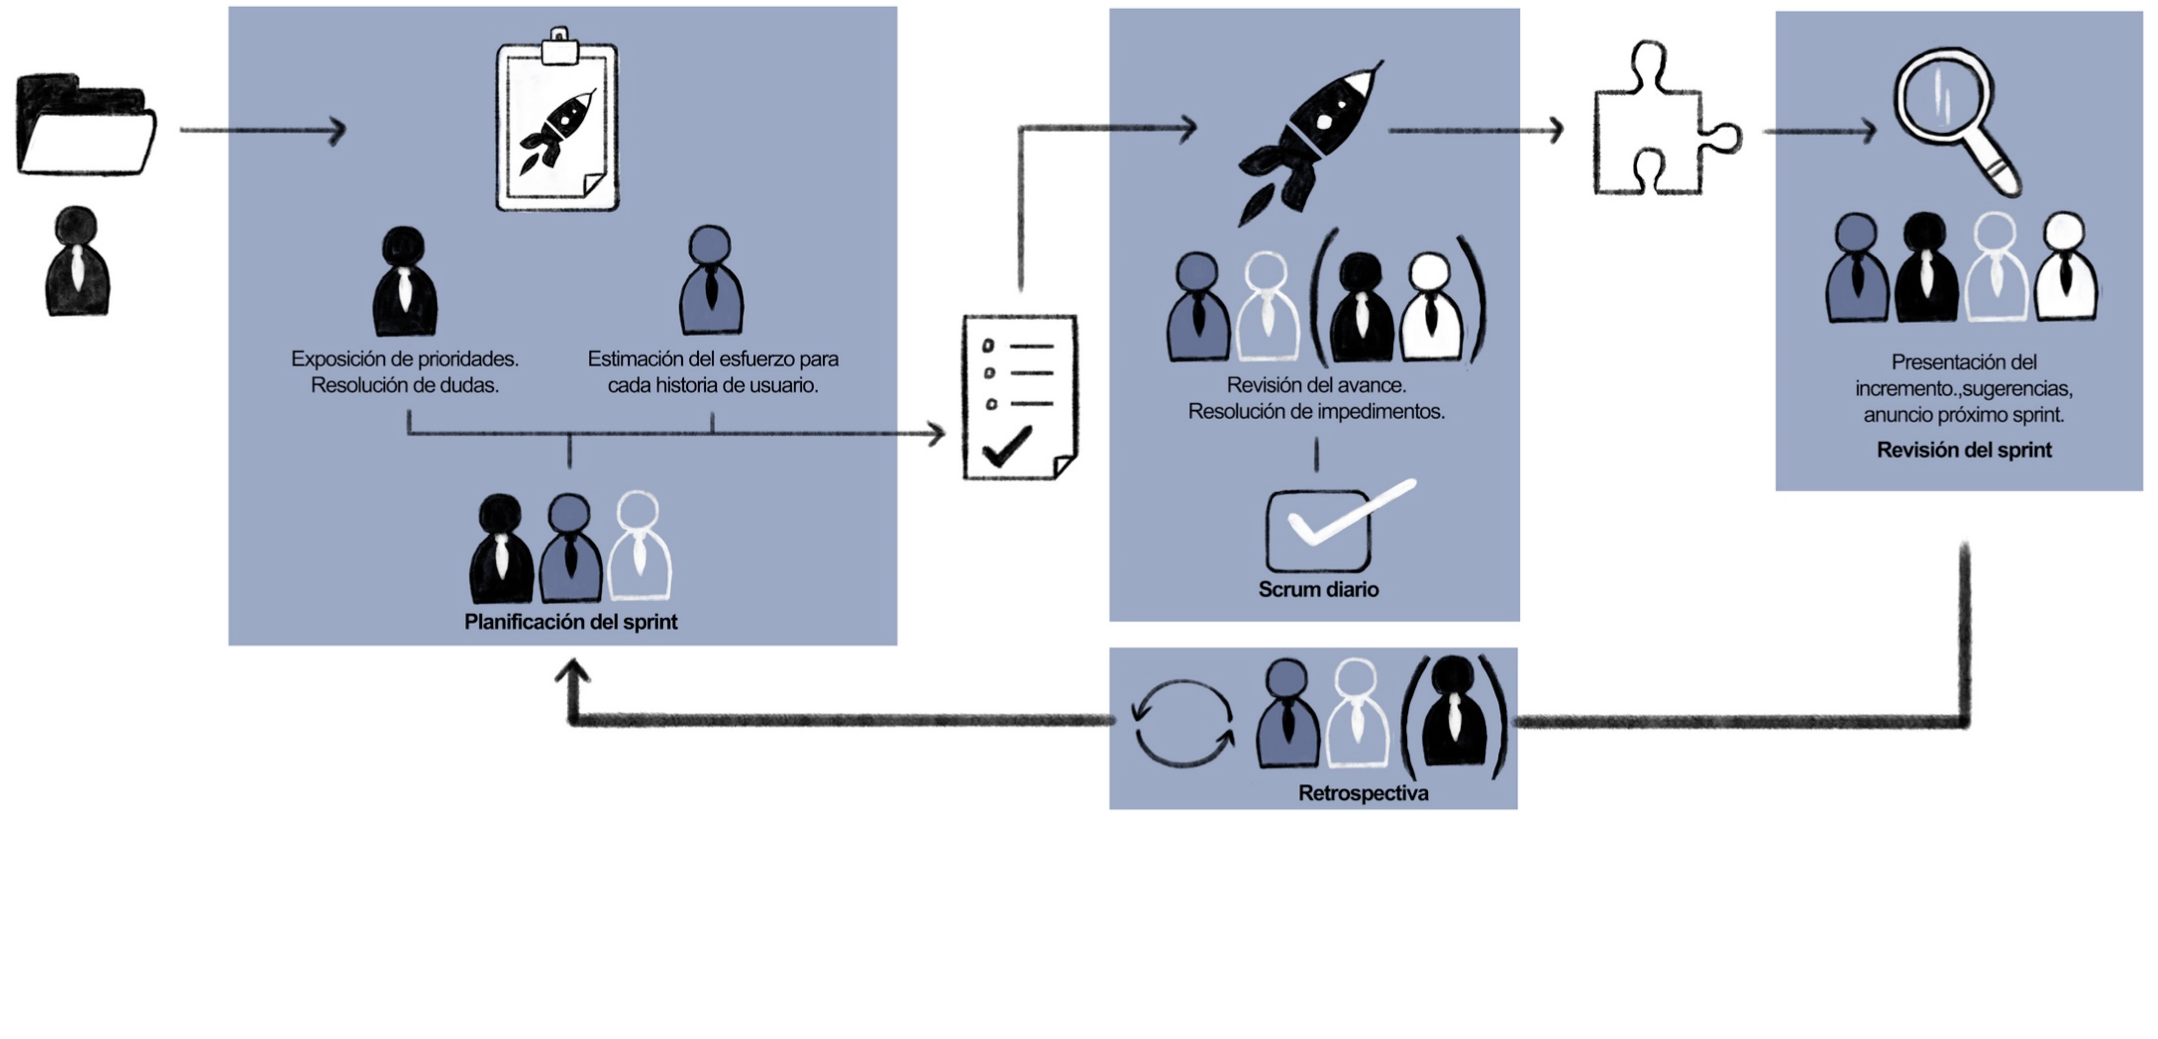
\includegraphics[width=\textwidth]{../img/Scrum/Scrum.png}
	\caption{\textit{Proceso seguido en Scrum \cite{scrum}}}\label{ProcesoScrum1}
\end{figure}


\begin{figure}
	\centering
	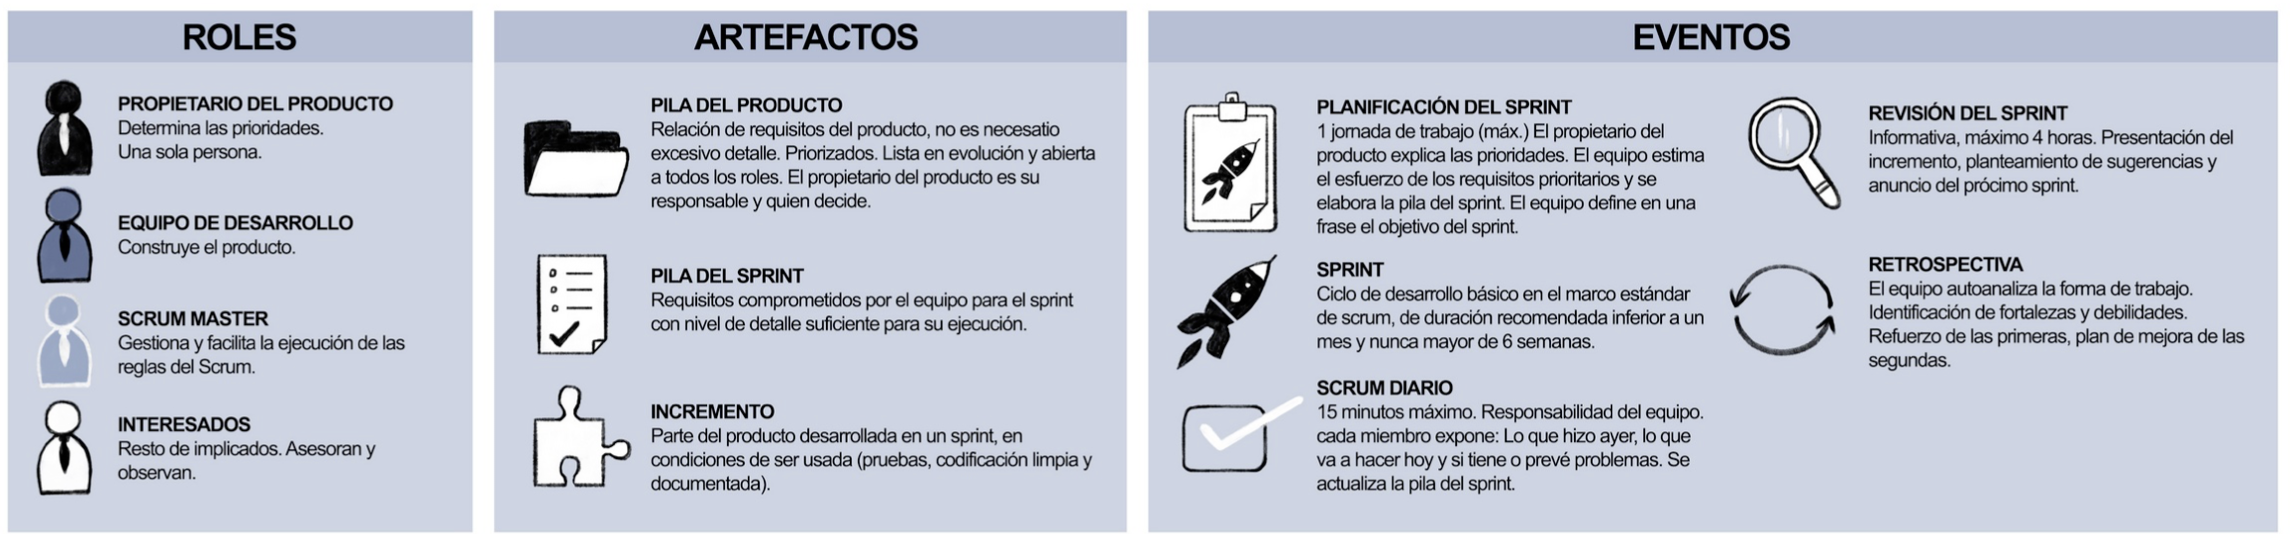
\includegraphics[width=\textwidth]{../img/Scrum/Scrum1.png}
	\caption{\textit{Explicación de los elementos del proceso \cite{scrum}}}\label{ProcesoScrum2}
\end{figure}


De forma resumida, para seguir la metodología Scrum es necesario que el propietario del producto genere inicialmente las historias de usuario, que se encontrarán en la pila del producto. Estas historias podrán aumentar a lo largo del desarrollo.

Con la pila del producto creada, todo el personal se reúne para planificar el \textit{sprint}. Estas reuniones son las que general la pila del \textit{sprint}.
Después de esta reunión, el equipo de desarrollo comienza a trabajar en las tareas que se ha comprometido para completarlas en el tiempo acordado. Cada día de trabajo se realiza una pequeña reunión de aproximadamente 15 minutos donde se expone el trabajo realizado, el trabajo que se va a hacer en el día, las dudas, etc., está reunión sirve para ir actualizando la pila del \textit{sprint}. 

Al final del \textit{sprint}, todo el personal se vuelve a reunir para presentar el incremento realizado y ver posibles cambios. Además, se fija el anuncio del próximo \textit{sprint} que comenzará de nuevo con una reunión de planificación.

Durante este proyecto se ha seguido una metodología Scrum con algunos cambios ya que no se hacían reuniones diarias ni los roles estaban tan marcados, pero la forma de trabajar era la misma con planificaciones y revisiones de \textit{sprints}.

\subsection{Web}
La web (\textit{World Wide Web}) es un sistema que permite la transmisión y acceso a datos y documentos a través de internet utilizando el protocolo HTTP para la comunicación y el lenguaje HTML para la representación de las páginas web~\cite{wiki:web}.

La tecnología web es una de las que más desarrollo ha sufrido en los últimos años. Esto ha provocado un cambio completo en nuestra forma de vida, afectando a aspectos como la búsqueda de información por Internet, realizar compras online, hacer trámites sin necesidad de acudir a una oficina, etc.,

 
\section{Herramientas}
\subsection{GitHub}
GitHub es una plataforma de alojamiento en la nube que permite llevar un control de versiones Git para los proyectos subidos. Además del control de versiones, GitHub posee distintas características como la creación de repositorios, el uso de \textit{issues}, \textit{Pull requests}, las páginas de \textit{wiki}, añadir distintos usuarios al repositorio con diferentes permisos, etc\cite{wiki:github}.

\subsection{ZenHub}
Extensión para navegador web que se integra con GitHub para permitir añadir los elementos de Scrum al repositorio. De esta manera se puede llevar un mejor seguimiento del trabajo realizado en el proyecto.

\subsection{Python}
Python es un popular lenguaje de programación que puede ser utilizado en diferentes ámbitos, entre ellos el desarrollo web. Algunas de las razones para utilizar este lenguaje es su facilidad de uso, la posibilidad de orientación a objetos y la amplia variedad de bibliotecas y frameworks, como puede ser Flask~\cite{python}.

Se estudió la posibilidad de uso de PHP para realizar la aplicación web, pero al final se decidió trabajar con Python debido a que es más conocido para los tutores del proyecto y a que, al utilizarlo durante el grado, es más fácil la adaptación para alumnos que en un futuro hagan nuevas versiones partiendo de este proyecto.

\subsection{Flask}
Como se ha comentado en el apartado anterior, Flask es un framework de Python que facilita la creación de aplicaciones web. Flask incluye el motor de plantillas Jinja2 que permite implementar código en las vistas de la aplicación de una forma cómoda y sencilla.

\subsection{JavaScript}
JavaScript es un lenguaje de programación interpretado débilmente tipado. Principalmente es conocido al ser utilizado en el lado del cliente para dar mejor interacción a páginas web estáticas, pero es mucho más potente de lo que se puede pensar y es utilizado en muchos más ámbitos. Incluso en la misma web, puede ser utilizado en el lado servidor mediante el entorno de ejecución Node.js. Esto permite que una aplicación web pueda estar completamente escrita en JavaScript~\cite{javascript}.

\subsection{HTML}
HTML es el <<Lenguaje de Marcas de Hipertexto>> utilizado por la \textit{World Wide Web} para representar las páginas web. Puede ser combinado con diferentes tecnologías como CSS para dar una apariencia diferente o JavaScript para poder interactuar de forma dinámica.

\subsection{CSS}
CSS, también conocido como <<Hojas de Estilo en Cascada>>, es un lenguaje de estilos utilizado para mejorar la apariencia de los ficheros HTML. Gracias a CSS se puede dar rienda suelta al diseño y hacer páginas web completamente diferentes.

\subsection{Bibliotecas / \textit{plugins}}
\begin{itemize}
\item\textbf{SQLAlchemy}

Biblioteca de SQL para Python que incluye una versión para el \textit{framework} Flask que permite su completa integración. 
SQLAlchemy contiene un conjunto de herramientas SQL que permiten el mapeo objeto-relacional, \textit{Object Relational Mapper (ORM)}. 
Esto permite que con un conjunto de expresiones requeridas por la biblioteca, se creen clases de objetos en Python que serán transformadas a tablas de una forma prácticamente abstracta para el desarrollador. 
Además, al estar los objetos vinculados a registros de una tabla SQL, cuenta con métodos para realizar distintas operaciones SQL como búsquedas, inserciones, eliminaciones, etc., sin tener que escribir sentencias SQL~\cite{sqlAlchemy}.

\item\textbf{Grid.js}

Grid.js es un \textit{plugin} de JavaScript que ayuda con el tratamiento de tablas. 
Gracias a esta biblioteca se pueden crear tablas con búsqueda, ordenamiento, redimensión de columnas, etc., de una forma sencilla gracias a sus herramientas. 
Además, Grid.js se puede incluir con \textit{frameworks} como Reac, Angular o Vue, pero también puede ser utilizado con JavaScript \textit{vanilla}.


Antes de la elección de este \textit{plugin} se estuvo valorando el uso de otro llamado DataTables. Al final se decidió utilizar Grid.js a pesar de que DataTables es más completo.

Algunas de las razones son la siguientes:
\begin{itemize}
\item Para utilizar Grid.js no es necesaria la biblioteca jQuery mientras que para DataTables sí. La dependencia de otras bibliotecas puede dar problemas en un futuro, además de que el rendimiento de JavaScript \textit{vanilla} es algo superior.
\item Aunque esto se pueda cambiar, la estética de Grid.js me parece más moderna.
\item Para este proyecto no eran necesarias muchas de las funcionalidades que aporta DataTables.
\item En su repositorio en GitHub, se puede ver por los \textit{commits} realizados que es un proyecto en continuo desarrollo.
\end{itemize}

\item\textbf{Select2}

Biblioteca de JavaScript que proporciona nuevas funcionalidades al campo \textit{select} de HTML. 
Gracias a esta biblioteca es posible escribir en el campo y realizar búsquedas más cómodas sobre los datos cargados en el campo.
Además, se pueden realizar consultas Ajax de los datos para no tener que realizar la carga completa de la información desde el inicio, sino que la información se va cargando según sea pedida por el usuario que maneja la aplicación.

\item\textbf{Sortable}
Se trata de una biblioteca de JavaScript que facilita la creación de listas con elementos arrastrables. También permite la ordenación en las listas creadas.

Esta biblioteca permite de una forma muy sencilla convertir listas estáticas de HTML en listas interactivas, lo que ofrece una gran personalización y posibilidades de manejo de la interfaz al poder gestionar los eventos de arrastrar o soltar elementos entre muchos otros. 
\end{itemize}

\subsection{Software}
\begin{itemize}
\item\textbf{Pincel Project}

Es un programa de ordenador gratuito y de código abierto que permite la creación de los prototipos de las vistas de una aplicación de una forma cómoda, arrastrando distintos elementos a la pantalla y modificándolos para que queden al gusto del creador. 
Cuenta con versiones para Windoes, Linux y macOS.
Por defecto, el software cuenta con objetos suficientes para crear los prototipos de las vistas de una aplicación. 
Sin embargo, es posible cargar más de estos objetos creados por la comunidad o por uno mismo, como pueden ser nuevos botones, campos de entrada, menús, etc.

\item\textbf{Draw.io}

Aplicación web que permite la creación de diagramas utilizando diferentes figuras geométricas. 
Además cuenta con objetos ya creados para crear diagramas utilizando UML, diagramas entidad-relación, diagramas relacionales, etc. 
Esta aplicación permite una personalización avanzada por lo que es muy útil para crear cualquier tipo de diagrama. 
Además, al ser una aplicación web no requiere de ningún tipo de instalación aunque si que cuenta con una versión de escritorio para Windows, Linux, macOS y Chrome OS.

\item\textbf{PyCharm}

Es un entorno de desarrollo integrado (IDE) que pertenece a la empresa JetBrains y que está creado para trabajar el proyectos basados en el lenguaje de programación Python. 
Cuenta con una licencia de uso gratuita con funciones limitadas, aunque para estudiantes regalan un año de licencia completa para todos los productos de la empresa.

PyCharm es uno de los IDE más completos y avanzados para el desarrollo con Python, ya que cuenta con una gran cantidad de características que facilitan el trabajo y ayudan a ahorrar tiempo. 
Además, a la hora de crear proyectos se puede indicar el tipo de \textit{framework} a utilizar, lo que hará que cargue de forma automática todos los paquetes necesarios y creará una versión simple del proyecto desde la que empezar a trabajar. 
Esto ahorra mucho tiempo al no tener que ir buscando e instalando los paquetes necesarios desde distintos repositorios. 
\end{itemize}
\subsection{}

\capitulo{5}{Aspectos relevantes del desarrollo del proyecto}

Este apartado pretende mostrar aquellos aspectos más relevantes del proyecto realizado.

\section{Diseño}
\subsection{Requisitos y casos de uso}
El proyecto realizado podría ser un buen ejemplo de un proyecto real en el que un jefe de proyecto debe comunicarse con el cliente para obtener los requisitos necesarios de la aplicación y trasladar la información requerida a desarrollar a los programadores (en este caso ambos roles los cumplía la misma persona).

La idea descrita anteriormente está motivada en que este proyecto se basa en una aplicación web que se pretende utilizar en la Universidad de Burgos. 
Por ello, los tutores del proyecto han actuado de una forma similar a clientes y durante las primera reuniones del proyecto daban la idea de como debía funcionar la aplicación a desarrollar.

El proceso de obtención de requisitos y diseño de casos de uso fue uno de los apartados de mayor duración del proyecto.
Esto es debido a que las primeras reuniones fueron dedicadas íntegramente a explicar la idea se tenía de cómo debía ser la aplicación web y qué requisitos era necesario cumplir.

En un principio se comenzó por ir diseñando el diagrama de entidad-relación.
De esta manera se veía de una forma más clara que entidades iba a tener la aplicación y cómo estas debían interaccionar entre ellas.
Este proceso duró varias semanas hasta dar con un diagrama que cumpliese de forma correcta con la idea de los tutores del proyecto y la idea que tenían de la aplicación web.

Con el diagrama de entidad-relación finalizado, se comenzaron a crear los diferentes casos de uso.
Este apartado del proyecto también tuvo una duración de varias semanas.
Durante este proceso se fueron creando todos los casos de uso de la aplicación, los cuales se pueden ver en los anexos.
Además, con la creación de estos se vieron algunos detalles que no estaban todavía bien especificados y debían determinar los tutores del proyecto.

Al cabo de varias semanas de diseño, cuando se tuvo una base correcta de trabajo, se comenzó con el prototipado de las vistas y, con el visto bueno de estas, el desarrollo del \textit{software}.

Cabe destacar que a pesar de haber hecho un largo proceso de diseño cuidando cada detalle, a lo largo del desarrollo hubo que retocar algún caso de uso o requisito para adaptarlo a nuevas necesidades surgidas que no se habían contemplado anteriormente o no se había profundizado lo suficiente en ellas.

\subsection{Interfaz}
Otro aspecto que se ha tenido muy en cuenta a la hora de desarrollar la aplicación es el diseño de la interfaz.

El diseño de las vistas ha intentado cuidarse para que fuese minimalista sin dejar que esto hiciese que se tuviese una \textit{web} poco atractiva.
La idea de hacer un diseño minimalista parte de principalmente de la idea de hacer más sencillo el uso de la aplicación al evitar elementos que desvíen la atención del usuario.
Además, el uso de un diseño minimalista ayuda a que la velocidad de carga de las páginas sea más rápida.
Estos dos elementos hacen que la experiencia del usuario al utilizar la aplicación \textit{web} sea mayor.

Otro aspecto que se ha cuidado al realizar la aplicación es que la web se adaptase lo máximo posible a cualquier tipo de resolución de pantalla, aspecto importante, ya que en esto es una mejora respecto a la aplicación SIGMA utilizada por la universidad.

Es necesario destacar que la aplicación \textit{web} desarrollada es funcional a través de cualquier dispositivo móvil, pero no se recomienda su uso de esta manera ya que la aplicación cuenta con grandes tablas que a pesar de adaptase a la pantalla, no son cómodas de manipular a través de este tipo de dispositivos.

\section{Desarrollo}
\subsection{Desarrollo web}
Como se ha comentado en la introducción, la aplicación desarrollada como proyecto ha sido una aplicación web.

Durante los cuatro años de estudio del grado apenas se han impartido lecciones sobre programación web, por ello, realizar una aplicación de este estilo supone invertir tiempo de aprendizaje previo a cualquier tipo de desarrollo.

En este caso, además se ha utilizado el \textit{framework} Flask que proporciona herramientas para facilitar la codificación, pero aun así, tiene una curva de aprendizaje necesaria antes de poder desarrollar código si se quieren seguir unas buenas pautas.

Creo necesario destacar este punto, ya que ha supuesto un trabajo adicional al tener que adquirir conocimientos acerca del desarrollo web.
Además, se ha intentado realizar una buena base para que alumnos en próximos cursos puedan tomar este proyecto y ampliarlo con más funcionalidades.
Para ello se han intentado plasmar las buenas prácticas aprendidas a lo largo de la carrera y durante el desarrollo.

\subsection{Inicio de sesión y las sesiones}
El inicio de sesión de la aplicación funciona mediante un formulario de correo electrónico y contraseña.
En un primer lugar se valida que el correo electrónico se encuentre en la base de datos propia y después se manda al Moodle de la Universidad de Burgos la petición mediante un \textit{endpoint} de su API. 
Si los datos son correctos se devuelve un \textit{token} que sirve para acceder a los recursos de Moodle.
En el caso de esta aplicación, el \textit{token} se guarda en la sesión para poder dar acceso al contenido de la misma.
Si en la sesión está el \textit{token} se permite el acceso, en caso contrario se redirige a la ventana de inicio de sesión.

La aplicación cuenta con un sistema de permisos que sólo permite acceder a aquellos usuarios con permisos de lectura y sólo permite modificar y ver cierta información a aquellos usuarios con permisos de modificación.

Para almacenar tanto el \textit{token} como el identificador del usuario, y así poder comprobar sus permisos, se hace uso de las sesiones.
Por defecto, la sesión se almacena en el cliente mediante una \textit{cookie}. 
El problema que tiene esta forma de trabajar es que la \textit{cookie} podría ser robada y con ello, el atacante podría tener acceso a la aplicación. 
En caso de guardar información sensible en la \textit{cookie} lo mejor es hacer el almacenamiento en el lado del servidor, y eso es lo que se ha hecho en esta aplicación para mejorar la seguridad.

\subsection{Creación de cursos académicos}
La creación de cursos académicos en la aplicación es una de las partes que más se ha cuidado debido a su importancia, ya que mientras algunos elementos, como por ejemplo los centros, lo normal es que se creen y no se vuelvan a tocar en mucho tiempo, la creación de cursos se realiza todos los años.
Además, crear un curso académico supone una carga de trabajo importante por parte del usuario, ya que debe seleccionar todas aquellas asignaturas deseadas para el curso, lo que puede ser un número elevado de elementos que se deben seleccionar de una forma cómoda.

Para resolver este problema en un principio se pensó en poner una tabla con todas las asignaturas existentes y un campo de selección, pero tras hacer una primera implementación de prueba se vio que no iba a ser algo cómodo para un uso real.
Tras investigar diferentes opciones se pensó en utilizar la biblioteca de JavaScript llamada <<Sortable.js>> que permite, entre muchas otras cosas, arrastrar elementos de la pantalla entre contenedores.
De esta manera se pueden tener las asignaturas que se desean seleccionar en un contenedor y las asignaturas seleccionadas en otro.

Finalmente, se decidió añadir un filtro por titulación y curso para que el usuario tenga un mayor control de las asignaturas a buscar y utilizar la biblioteca \texttt{Sortable.js} para permitir arrastrar las asignaturas requeridas de forma simultanea.
Al arrastrar, estas son seleccionadas para añadir al curso.

Esta forma de trabajar hace que la aplicación se maneje de una forma más cómoda y dinámica que si se hubiesen usado otras opciones.
Además, se añadió la opción de duplicar un curso académico completo para que de un año a otro no haya que crear todas las vinculaciones si no que se pueda partir de las asignaciones realizadas en cursos previos.

\subsection{Importaciones seguras de datos}
La aplicación web desarrollada permite importar datos a la base de datos.
Esta funcionalidad está diseñada para facilitar la instalación de la aplicación en diferentes ubicaciones, ya que permite introducir datos directamente, de forma masiva, evitando la necesidad de crearlos manualmente.

La forma de trabajar de esta funcionalidad es permitir únicamente ficheros \texttt{SQL} con sentencias \texttt{INSERT}. 
Si incluye cualquier otro tipo de sentencias, estas serán rechazadas.
Esto se debe a que el propósito de este sistema es permitir la inserción de datos en la base de datos, pero nada más.
De esta forma, se garantiza que la importación se realice de una forma segura, evitando cualquier tipo de sentencia que pueda dañar el contenido de la base de datos.

A pesar de todo, se trata de una operación compleja, por lo que se recomienda realizar una exportación de los datos o una copia de seguridad previamente.

\subsection{Modificación de horas desde la tabla}
La asignación de horas de una plaza a un grupo de una asignatura durante un curso académico es una de las tareas más habituales y tediosas a la hora de trabajar gestionando el PDI. 
Por ello, se ha intentado hacer que esta labor sea lo más cómoda posible.

Se ha implementado la funcionalidad de poder realizar la asignación de horas directamente desde la tabla donde se muestra esta información permitiendo la navegación entre campos mediante el tabulador.

El funcionamiento se basa en modificar los campos de <<Horas en el grupo>> desde la tabla general donde se muestran todos los grupos de un curso junto a las plazas vinculadas. 
La asignación de horas se realiza al momento de perder el foco del campo sin necesidad de recargar la página gracias al uso de peticiones asíncronas mediante AJAX.
Además, se realiza la actualización de la columna <<Horas totales asignadas>> también de forma automática.

Esto facilita mucho la modificación de horas y hace que la forma de trabajar sea similar, salvando las distancias, a una hoja de cálculo (como por ejemplo Microsoft Excel).


\capitulo{6}{Trabajos relacionados}

A continuación se presentarán diferentes trabajos que mantienen relación con la aplicación desarrollada en este trabajo de fin de grado.
Estos trabajos han abordado diferentes aspectos relacionados con la gestión del personal, principalmente desde el punto de vista la planificación y asignación de recursos.

\begin{itemize}
\item \textbf{SIGMA}\footnote{\url{https://www.sigmaaie.org/es}}\label{SIGMA}

SIGMA es un \textit{software} diseñado para la gestión académica y es utilizado por un gran número de universidades españolas, entre ellas la Universidad de Burgos.
Está diseñado para ayudar a las instituciones educativas a gestionar tanto sus procesos administrativos como académicos.
Esto incluye, entre otras, la gestión de estudiantes, docentes, matrículas, cursos académicos y calificaciones.

Esta plataforma es muy completa ya que permite gestionar prácticamente todo el ciclo de vida de la gestión académica. Sin embargo, cada institución tiene sus propias particularidades y ahí es donde la aplicación de este trabajo destaca por completo al estar hecha a medida para lo que se requiere.

A día de hoy SIGMA cuenta con algunas desventajas que hacen que su uso no sea del todo cómodo.
Algunas de estas son que cuenta con un diseño pensado para pantallas grandes que no se adapta bien a otro tipo de resoluciones, es decir, un diseño no \textit{responsive}, se encuentra migrada a una aplicación web de una mala manera ya que su funcionamiento es lanzando procesos en una web, no visualiza fácilmente la información en pantalla sino que se basa en listados de generación asíncrona y cuenta con problemas de integración.

\item \textbf{Classter}\footnote{\url{https://www.classter.com/}}

Es una plataforma de gestión académica que permite controlar el proceso educativo al completo.
Incluye un sistema para la gestión de estudiantes, profesorado, aulas, calificaciones, etc.

Los puntos fuertes de esta plataforma podrían ser su modularidad, que permite añadir sólo aquellas partes que se deseen, la personalización, que permite adaptar la aplicación a cada institución y la facilidad de comunicación que proporciona entre docentes y alumnos.

Entre sus principales desventajas se encuentran una gran curva de aprendizaje, es decir, que cuesta conocer y trabajar con normalidad con el sistema desde un principio y requiere de un proceso de aprendizaje previo para aprovecharlo al completo, la falta o mala integración con otras herramientas para la gestión académica y por último, el costo.

\item \textbf{Constructor}\footnote{\url{https://constructor.tech/solutions/higher-education}}

Constructor es una plataforma pensada para instituciones de educación superior.
Ofrece diferentes soluciones entre las que se encuentran la gestión del PDI, la administración de cursos, una plataforma de enseñanza \textit{online} y la gestión de servicios estudiantiles como pueden ser matrículas, biblioteca, gestión de becas, etc.


\end{itemize}

\capitulo{7}{Conclusiones y Líneas de trabajo futuras}

Para finalizar la memoria de este proyecto, se va a hacer una valoración final del trabajo realizado y los conocimientos adquiridos durante el proceso.

También se van a indicar nuevas funcionalidades que podrían ser interesantes para la aplicación desarrollada y que harían esta herramienta un \textit{software} mucho más completo.

\section{Conclusiones}
Este trabajo de fin de grado pone punto final a cuatro años de formación y aprendizaje, no solo el desarrollo de \textit{software}, si no de haber adquirido una visión crítica sobre cualquier fase del ciclo de vida de un proyecto, enfocado sobre todo al ámbito de la informática.

La realización de este trabajo ha permitido plasmar la capacidad adquirida de adaptación a cualquier tipo de lenguaje o tecnología, y la aptitud de seguir el proceso de desarrollo de un proyecto desde su diseño hasta su despliegue.

La redacción de la documentación ha sido una de las partes que más recursos temporales ha consumido, pero que es necesario para plasmar el trabajo realizado, los conocimientos adquiridos y marcar unas líneas de trabajo y manuales para que futuros alumnos puedan continuar con el desarrollo de este proyecto.

"Considero importante resaltar el trabajo de investigación y aprendizaje llevado a cabo durante el proyecto, incluso antes de su asignación oficial.
Las investigaciones realizadas no han sido sobre artículos u otros trabajos anteriores, sino que se ha realizado un proceso de investigación de herramientas y técnicas que podrían resultar útiles, así como el aprendizaje de su correcto uso.

Durante la vida del proyecto también se han tenido que aprender y aplicar buenas técnicas de programación para intentar hacer el código lo más accesible, mantenible y escalable posible.

Además de todo lo anterior, el desarrollo web es una parte de la informática que se aborda en menor medida a lo largo de la carrera. Por lo tanto, llevar a cabo un proyecto que se centre principalmente en el desarrollo web implica la necesidad de aprender sobre este tema en poco tiempo.


\section{Líneas de trabajo futuras}
A continuación, se expondrán una serie de mejoras que podrían llevar a la aplicación a un nivel aún más completo.

\subsection{Cambios en las áreas}
Posiblemente será necesaria una modificación del diseño de áreas debido al cambio que se pretende introducir con el <<Proyecto de Real Decreto por el que se establecen los ámbitos de conocimiento a efectos de la adscripción de los puestos de trabajo del profesorado universitario>>~\cite{gob:areas}. 

Entre las medidas incluidas en el proyecto, se encuentra una que pretende cambiar el nombre que reciben las áreas en la descripción de las plazas de profesorado.

\subsection{Creación avanzada de grupos}
En la actualidad, los grupos se generan automáticamente con un nombre basado en su tipo (teórico o práctico) y modalidad (online, presencial o en inglés). Este enfoque asegura el uso correcto de los códigos de grupo y mantiene una proporción adecuada entre los grupos teóricos y prácticos.

No obstante, sería interesante considerar la adición de una funcionalidad que permita elegir la forma de crear un nuevo grupo. De esta manera, se podría mantener el sistema actual, al mismo tiempo que se incorporaría una nueva opción que permita agregar un grupo manualmente mediante la introducción del código correspondiente, sin afectar al resto de los códigos de grupo.

\subsection{Añadir gráficas}
La aplicación desarrollada permite obtener diversos datos, como las horas que un docente imparte en un curso o titulación, la cantidad de plazas por cada tipo de contrato o el número de contrataciones en un rango de fechas, entre otros.

Toda esta información podría ser representada en diferentes gráficas. Además, sería posible hacer que estas gráficas sean interactivas, permitiendo al usuario agregar o eliminar fuentes de datos para obtener la representación gráfica deseada.

Considero que esta mejora sería muy interesante, ya que proporcionaría información de manera más rápida y visual que en la configuración actual.

\subsection{Integración con Moodle}
Otro aspecto que podría ser muy interesante desarrollar es buscar la manera de integrar esta aplicación con Moodle, la plataforma utilizada por la universidad.

Moodle ofrece una API que permite realizar diversas acciones. 
Sería beneficioso explorar en mayor profundidad esta API para determinar la posibilidad de recuperar información relevante del Moodle, como datos de docentes, titulaciones, asignaturas, entre otros. 
Asimismo, se podría agregar nueva información a la aplicación que también pudiera obtenerse desde esta plataforma.

Por otro lado, se podría estudiar la funcionalidad inversa, es decir, la capacidad de enviar datos desde la aplicación web desarrollada hacia Moodle.
De esta forma se podría, por ejemplo, realizar la planificación de un curso académico desde esta aplicación y que se replique de forma automática en Moodle.

Cabe destacar que esta nueva funcionalidad requeriría un estudio e integración exhaustivos, ya que es probable que los datos no se envíen en el mismo formato y se requieran diferentes soluciones.
No obstante, creo que podría ser una característica muy cómoda para el uso real de la aplicación.

\subsection{Generación de horarios}
Una interesante adición sería la capacidad de generar horarios dentro de la aplicación. 
Gracias a la información proporcionada sobre titulaciones, asignaturas y grupos asociados, sería posible generar automáticamente un horario que aportando las horas de las clases.

Además, al especificar los docentes asignados a cada grupo desde la aplicación, también podrían aparecer en el horario correspondiente. 
Esto permitiría generar un horario completo que, incluso, podría convertirse a formato PDF para facilitar su visualización y distribución.





\bibliographystyle{plain}
\bibliography{bibliografia}

\end{document}
